\documentclass{article}
\usepackage[utf8]{inputenc}
\usepackage[spanish]{babel}
\usepackage{listings}
\usepackage{graphicx}
\graphicspath{ {images/} }
\usepackage{cite}

\begin{document}

\begin{titlepage}
    \begin{center}
        \vspace*{1cm}
            
        \Huge
        \textbf{Taller No. 1}
            
        \vspace{0.5cm}
        \LARGE
        Nociones de la memoria del computador
            
        \vspace{1.5cm}
            
        \textbf{Carlos Alfredo Pinto Hernández}
            
        \vfill
        
        \vspace{0.8cm}
            
        \Large
        Departamento de Ingeniería Electrónica y Telecomunicaciones\\
        Universidad de Antioquia\\
        Medellín\\
        Septiembre de 2020
            
    \end{center}
\end{titlepage}

\tableofcontents

\section{Introducción}
En la actualidad, en la mayoría de hogares se dispone de un computador para la realización de diferentes actividades, desde editar un documento hasta jugar videojuegos, estos dispositivos se han vuelto parte esencial en cada una de las familias debido a brinda soluciones o entretenimiento a todos los integrantes del hogar.\\\
El funcionamiento de un computador esta determinado por una interrelación de componentes físicos (hardware) como no tangibles (software). Uno de los componentes más importantes del hardware es la memoria y es este dispositivo el que presentan grandes funcionalidades para el correcto funcionamiento del computador.\\\
A continuación, se describe el concepto de memoria, su clasificación, la gestión de memoria y unos conceptos relacionados con la velocidad de procesamiento de las memorias.


\section{Desarrollo} \label{contenido}
\subsection{Memoria}
Es el componente imprescindible del computador que mantiene disponibles las instrucciones para el microprocesador pueda ejecutarlas, además se encarga de almacenar temporalmente el resultado de los procesos ejecutados.\cite{EcuRed}

La memoria juega un papel importante en la ejecución de las diversas tareas que son requeridas por el sistema operativo o el usuario, es el espacio en el que se ubican los datos de los procesos a ejecutar en nuestro computador de manera temporal.

Otra definición más técnica podría ser considerar a la memoria como un dispositivo de almacenamiento temporal y alta velocidad de acceso (ej. memoria principal del computador)\cite{Academia}

\subsection{Tipos de memoria}
Existe una jerarquía de memorias en la cuales se clasificación según sus características: capacidad de almacenamiento, velocidad y costo. Esta clasificación tiene un objetivo principal y es conseguir que, cuando el procesador acceda a un dato, este se encuentre en el nivel más rápido de la jerarquía.\cite{Estructura}

La Figura (\ref{fig:Jerarquia}) describe un esquema de la jerarquía de memoria en el computador.
A continuación se describen los principales tipos de memorias con sus características.

\begin{figure}[h]
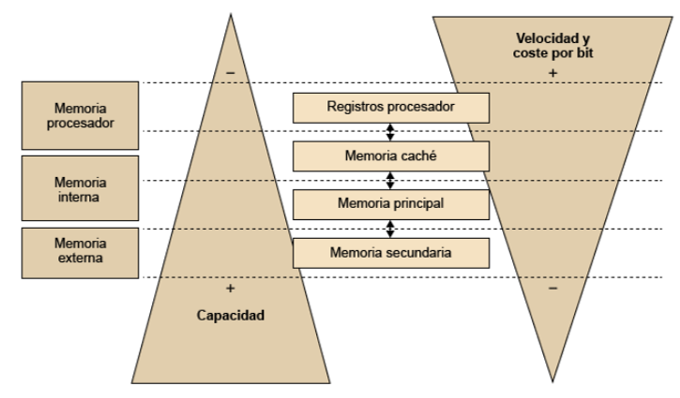
\includegraphics[width=10cm]{Jerarquia.png}
\centering
\caption{Jerarquía de memorias}
\label{fig:Jerarquia}
\end{figure}

\subsubsection{Memoria Caché}
Son dispositivos de capacidad reducida pero de gran velocidad. Se suele encontrar dentro del procesador y están diseñadas para reducir el tiempo de acceso a la memoria. En este dispositivo se almacenan los datos o instrucciones más utilizadas por el procesador. \cite{Estructura}

A su vez se divide en 3 niveles (l1, L2 y L3), el primer nivel está dividido en memoria de instrucciones y memoria de datos. Las últimas dos son unificadas.

\subsubsection{Memoria RAM o principal}
En la memoria principal se almacenan los programas que se deben ejecutar y sus datos, es la memoria visible para el programador mediante su espacio de direcciones.
La RAM es utilizada tanto para almacenar datos como para almacenar los programas en uso. La velocidad de la RAM en la mayoría de los sistemas actuales está entre la velocidad de la memoria caché y la de los discos duros y está mucho más cercana a la velocidad de la primera que a la segunda.\cite{MIT} \break
La memoria principal tiene una capacidad mucho más elevada que la memoria caché (del orden de Gbytes o de Tbytes en supercomputadores). Utiliza tecnología DRAM (Dynamic RAM), que es más lenta que la SRAM, pero con una capacidad de integración mucho más elevada, hecho que permite obtener más capacidad en menos espacio.\cite{Estructura}

\subsubsection{Memoria Virtual}
Es una parte del disco duro designada exclusivamente para soportar partes de programas o datos que están en ejecución y que el momento no se están ejecutando pero en algún momento lo hará. De esta forma se libera al programador de las restricciones de la memoria principal.

\subsubsection{Memoria Externa}
Esta clasificación corresponde a dispositivos de almacenamiento secundario y también se pueden considerar sistemas de almacenamiento en red. Los dispositivos que forman la memoria externa se conectan al computador con algún tipo de bus (serie o paralelo). Estos dispositivos se pueden encontrar físicamente dentro del computador conectados por buses internos del computador (IDE, SATA, SCSI, etc.) o pueden estar fuera del computador conectados por buses externos (USB, Firewire, eSATA, Infiniband, etc.).\cite{Estructura}\\

\textbf{Conocimientos previos: }De los diferentes tipos de memorias mencionadas anteriormente, antes de la realización de la investigación solo conocía la memoria RAM y el disco duro.

\subsection{Gestión de memoria}
La correcta gestión de memoria es muy importante debido a que la correcta utilización de esta permitirá realizar todas las tareas asignadas de manera eficiente en el computador. Existen múltiples técnicas de gestión de memoria, a continuación se describen de manera resumida las principales, incluyendo las primeras técnicas definidas.\cite{Gestion}

\subsubsection{Sistemas Primitivos}
Es el almacenamiento más simple en cuando a soporte hardware y necesidades de gestión. El \underline{monitor residente} consistía en cargar un único programa en memoria. La otra forma era la denominada \underline{particiones} que permitía gestionar varios programas asignado un espacio contiguo a cada uno. Se puede hacer la particiones de dos formas de tipo fijo o variable.

\subsubsection{Swapping}
Es el mecanismo para mover programas entre la memoria principal al disco duro, de esta forma los programas pueden entrar/salir de la memoria durante el tiempo de ejecución. Las principales ventajas de esta técnica es que permite influir en la gestión de procesos para controlar el grado de multiprogramación y proporciona flexibilidad en la gestión de la memoria, permitiendo una utilización más eficiente del espacio.

\subsubsection{Paginación y segmentación}
Esta técnica permite la ubicación no contigua de programas con el fin de combatir la fragmentación y la degradación de la memoria. Al poder ubicarse de forma no contigua, un programa ya no necesita un espacio de su tamaño, sino que la cantidad total de memoria libre sea mayor o igual.

\subsubsection{Enlace Dinámico}
Hace referencia a la técnica en la cual se divide el programa en varios módulos a partir de su estructura y cargar de forma dinámica solo aquellos que se necesiten.
\subsubsection{Memoria Virtual}
Es el mecanismo más general para la ejecución de programas no enteros en memoria. Se basa en un sistema de paginación (o combinado) en el que sólo un subconjunto de las páginas del programa están cargadas en memoria y el resto reside en un dispositivo de almacenamiento secundario.

\subsection{Velocidad de memoria}
\textbf{¿Qué hace que una memoria sea más rápida que otra?}\\
La velocidad de memoria está relacionada por la latencia o tiempo de acceso, la cual se define como el tiempo que transcurre desde que una dirección de memoria es visible para los circuitos de la memoria hasta que el dato está almacenado (escritura) o está disponible para ser utilizado (lectura); lo anterior para memorias de acceso aleatorio. En memorias de acceso no aleatorio la latencia es el tiempo necesario para que el mecanismo de lectura o escritura se sitúe en la posición necesaria para empezar la lectura o escritura.\cite{Estructura}\\
Otro concepto es el de tiempo de ciclo de memoria el cual se define como el tiempo de acceso más el tiempo necesario antes de que se pueda empezar un segundo acceso a la memoria.\\\
Por ultimo se define la velocidad de transferencia de memoria como la velocidad a la cual se puede leer o escribir un dato en memoria. Y este será el inverso del tiempo del ciclo. La velocidad de transferencia se mide en bytes por segundo; es habitual indicar la velocidad de una memoria en MB/segundo o GB/segundo.\\

\textbf{¿Por qué esto es importante?}
Al conocer estos conceptos podemos comprender el funcionamiento de la memoria y de esta forma generar procesos para su uso eficiente, evitando uso innecesario de la memoria en la ejecución de programas. Disponer de una mayor velocidad permitirá realizar múltiples actividades de manera rápida ya que se realizan las transferencias de datos e instrucciones en menos tiempo. 


\section{Conclusiones} \label{conclusion}
\begin{itemize}
  \item La memoria en el computador juega un papel crucial en el funcionamiento de este, debido a que permite almacenar de forma temporal la información utilizada por el procesador para generar los resultados que el usuario final requiere.
  \item Existe una jerarquía de memoria donde se relaciona su capacidad versus su velocidad, las cuales son inversamente proporcionales. Siendo las de menor capacidad y mayor velocidad las memorias caché y en el otro extremo las memorias externas con mayor capacidad, pero menor velocidad.
  \item La correcta gestión de memoria permitirá potencializar los recursos de memoria y de manera directa mejorar el funcionamiento del computador para hacer las tareas requeridas de manera más eficiente.
  \item Como ingenieros es importante afianzar estos conocimientos ya que pueden ser de gran utilidad a la hora de programar y hacer más eficiente el uso de memoria y de esta forma generar programas que puedan ser diferenciadores y sostenibles en el tiempo.
\end{itemize}

\bibliographystyle{IEEEtran}
\bibliography{references}

\end{document}
